\documentclass[conference]{IEEEtran}
\IEEEoverridecommandlockouts
% The preceding line is only needed to identify funding in the first footnote. If that is unneeded, please comment it out.
\usepackage{cite}
\usepackage{amsmath,amssymb,amsfonts}
\usepackage{algorithmic}
\usepackage{graphicx}
\usepackage{textcomp}
\usepackage{xcolor}
\def\BibTeX{{\rm B\kern-.05em{\sc i\kern-.025em b}\kern-.08em
    T\kern-.1667em\lower.7ex\hbox{E}\kern-.125emX}}
\begin{document}

\title{Plant Detection, Plant Segmentation and Leaf Instance Segmentation}


\author{\IEEEauthorblockN{ Tianyi Wu, Siyu Gao, Xiaole Du, Gewei Cheng, Lijun Zhong}
\IEEEauthorblockA{\textit{University of New South Wales} }
}

\maketitle

\begin{abstract}
This project compared several methods based on given image datasets to achieve plant detection, plant segmentation, and leaf instance segmentation, comparing the impact of different methods with measures.
\end{abstract}

\begin{IEEEkeywords}
Plant Detection, Plant Segmentation, Leaf Instance Segmentation, HOG, SVM, K-means, Watershed, Color Threshold, MASK-R-CNN.
\end{IEEEkeywords}

\section{Introduction}
For the development of human society, the plant is widely considered to be the most closely related species on the earth. 
Plants provide the basic source of carbohydrates and are also the source of feed for animal husbandry. 
The most basic characteristic of plants is the leaf. 
Therefore, the establishment of a cognitive system for plant species, maturity, growth rules, etc., is the prerequisite for the human to conquer nature. 
Based on the knowledge of computer vision, this project strives to correctly process the pictures of plants such as Arabidopsis and tobacco. 
The Color Threshold and HOG+SVM are used to correctly detect the position of the plant in the picture in task 1, the average precision reaches 90\%; 
through methods such as Kmeans and Watershed, task 2 achieve the extraction of plant leaf information, the Dice similarity coefficient and intersection over union measures of identifying the leaf area reached 94\%; 
furthermore, applying the MASK-R-CNN method, task 3 identified and segmented different leaves and labeled leaf instances, The symmetric best dice measure reached 79\%. 
The data sets used in this project comes from CVPPP.

\section{Literature Review}
For plant detection, we applied HOG+SVM and Color Thresholding.
Histograms of oriented gradients is a commonly used method for detecting objects (especially pedestrians)[9], which applies histograms of oriented gradients for feature generation, as well as Support Vector Machine classifier for functional classification.
As SVM is a time-consuming classifier, one project from a group delivered an approach with HOG and predicting SVM results without too much resource usage[10]2.
Besides, sliding windows are utilized in this task to detect plant. And Zhang et al. [11]3 have imaged a method with a coarse-to-fine feature hierarchy, which decreases the possibility of presenting negative windows.
And these methods will be implemented and evaluated.

For plant segmentation, There are some studies that have demonstrated the segmentation methods of living plants from whose background using unsupervised [12,13] and semisupervised algorithms [14]. 
K-means algorithm is a commonly used method for image segmentation is the most popular method for image segmentation [16][17][18], since it could cluster a great number of data points in a short time [19].
Leaf segmentation could be achieved through watershed segmentation [15] applying the obtained initial seeds over the image space. 
However, there is still quite of work to be evaluated with different measures.

In instance segmentation, multiple task networks have become mainstream in recent years. there are two main methods. The first one is the bottom-up method based on semantic segmentation. The second one is the top-down method based on the detection. Some method uses the Lab color space of the 3D histogram to segment background and foreground, and then mathematical methods are used to extract the center of leaf from the foreground. These centers are used for instance segmentation.[4] In the first method, semantic segmentation from the image firstly, and then use the discriminant loss function for training, and finally use some clustering method to clustering different instances.[3] The other one is to find the bounding box where the instance is located, and then semantic segmentation in the bounding box, and then output the segmentation results as different instances[1]. Most of these methods are using deep learning. However, deep learning needs a large amount of data for training. The collection of data may costly and a waste of time. Some effective strategies are used to overcome these drawbacks, such as: synthetic dataset[7] and transfer learning[8].

\section{Methods}

\subsection{NormalizedRGB and HSV}
The RGB color space applies a linear combination of three color channels to represent colors. Any represented color is related to these three components, and they are highly correlated. Therefore, it is not intuitive to continuously change colors. Adjustments need to be implemented on that. 
By observing the input data of this task, it can be found that the natural lighting, occlusion, and shadows in the photo make a greater impact on the brightness of different parts of the picture.

However, since the RGB color space is greatly affected by the illumination, to reduce the influence of it, the normalization process is first performed in the RGB space. That is, the green component g, red component r, and blue component b are extracted from the image, which is normalized to R, G, and B (see equation (1)). To distinguish the green characteristics, using the (-1 , 2, -1) mask template to process the channels (R, G, B) at each point of the image, as shown in equation (1). The template emphasizes the green component, suppresses the red and blue components, and the template sum is zero. Which makes it symmetrical, and the length is odd, so it has a linear phase, which guarantees the time-invariant requirement. 

\begin{equation}
\begin{aligned}
G= {\frac{g}{g+r+b}}\\ R={\frac{r}{g+r+b}}\\ B={\frac{b}{g+r+b}}
\end{aligned}
\end{equation}

$$
ROI=\begin{bmatrix} -1 & 2 & -1  \end{bmatrix} * \begin{bmatrix} R \\ G \\ B  \end{bmatrix}
$$

In the RGB color space, all three color components are closely related to brightness. In other words, as long as the brightness changes, they will change accordingly, and there is no more intuitive way to express the same channel. Since all image processing approaches should be accessed by human eyes. In monochrome, eyes are the least sensitive to red and the most sensitive to blue, so the RGB color space is a color space with poor uniformity. If the similarity of colors is directly measured by Euclidean distance, the result will have a large deviation from human vision. For a certain color, it is difficult to infer a more accurate three-component value to represent.

For these tasks, there will be a big difference between the leaves of the plants and the background tray. The direct difference of the plant leaves is only reflected in the color tone, brightness, and saturation. For further identification of leaf area grown condition and maturity also depends on these key parameters. In this project, there are some horizontally compared results between two different color space formats regarding the accuracy of identification as well as prediction.

Based on the above reasons, the HSV color space is more commonly used in image processing, which is closer to human perception than RGB. It is very intuitive to express the hue, vividness, and brightness of the color, which is convenient for color contrast. In HSV color space, it is easier to track objects of a certain color than BGR, and it is often used to segment objects of the specified color.


\subsection{Morphological processing}
The image processed by the above methods will still have some stray points shown. At this time, the open operation in the morphological algorithm can be used to remove [10]:
	
The opening operation of the structural element B on image A is denoted as $A \circ B$, as shown in formula (2), the image is first corroded and then expanded. Corrosion could help to remove stray points, but also make the edge area smaller, so it needs to be restored by expansion.
\begin{equation}
A \circ B = ( A \Theta B ) \oplus B
\end{equation}

Corrosion is denoted as $A\Theta B$, as shown in formula (3), where $A^{C}$ is the complement of $A$, and $\emptyset$ is the empty set.
\begin{equation}
A\Theta B = \{ z | {(B)}_{z} \cap A^{C} \neq \emptyset) 
\end{equation}

The expansion is denoted as $A\oplus B$, as shown in equation (4), 
where $\hat{B}$ is the symmetrical image of $B$ about the origin, $\emptyset$ is the empty set.

\begin{equation}
A\oplus B = \{ z | {(\hat{B})}_{z} \cap A \neq \emptyset) 
\end{equation}

\subsection{HOG and SVM}
The target detection task involves determining the presence of a target in an image and its location. HOG is a histogram of gradient-based feature descriptors, which is often used in face recognition to compute and count histograms of gradient directions in localized areas of an image to form features.
When computing the HOG Descriptor, there will be the following parameters. windowSize, blockSize, blockStep, cellSize, binNum. Each window will be divided into blocks, and each block will be divided into cells. nbins represent the number of directions of a statistical gradient in a cell. A histogram of the gradient of each pixel in the cell unit is captured. Finally, these histograms are combined to form a feature descriptor.\\		
The number of cells in a block is:


\begin{equation}
A = {\frac{blockSize.width}{cellSize.width}}* {\frac{blockSize.height}{cellSize.height}}
\end{equation}

Each block contains $binNum*A$ gradient histogram.\\
The number of blocks in a window is:\\

\begin{equation}
\begin{aligned}
B= {\frac{windowSize.width-blockSize.width}{blockStep.width+1}}\\ *  {\frac{windowSize.height-blockSize.height}{blockStep.height+1}}
\end{aligned}
\end{equation}

One window contains 9AB gradient histograms. There are two other issues that need to be solved when using hog: scale and position. The scale problem can be solved by resizing the image. To solve the position problem, image pyramids and sliding windows are used.

\subsubsection{Image Pyramid}

An image pyramid is a multi-scale representation of an image, which helps solve the problem of target detection at different scales. The more layers of the pyramid, the slower the computation will be, but the more accurate the results will be to some extent.


\subsubsection{Sliding window}

Setting the window size to slide in the image, sliding window detection, and using the image pyramid to detect each part, is to detect objects at multiple scales. The sliding window solves the localization problem by scanning smaller areas of a larger image and thus repeating the scan at different scales of the same image. However, there is also the problem of region overlap, which requires non-maximal suppression to solve.

\subsubsection{non max suppression}

Non-maximal suppression is widely used in calculator vision tasks. Since in target detection, multiple candidate boxes are often generated for the same target, and they overlap. It is necessary to use non-maximal suppression to find the best target candidate frame and remove the redundant candidate frames.

After HOG, a classifier is needed to classify the features. Generally, support vector machine (SVM) will be chosen.
In machine learning, a support vector machine (SVM) is a supervised learning model and associated learning algorithm for analyzing data in classification and regression analysis. Given a set of training instances, each of which is labeled as belonging to one or the other of two categories, the SVM training algorithm creates a model that assigns new instances to one of the two categories, making it a non-probabilistic binary linear classifier.


\begin{itemize}
\item Scale-space extreme value detection: construct Gaussian pyramids, Gaussian difference pyramids, and detect extreme points.
\item Keypoint positioning: remove the influence of small contrast and edges on extreme points.
\item Determine the direction of key points: Use gradient histogram to determine the direction of key points.
\item Keypoint description: block the image area around the key point, calculate the gradient histogram within the block, generate feature vectors, and describe the key point information.
\end{itemize}

\subsection{K-Means Clustering Algorithm}
In this project, it is not difficult to check all the input pictures and find that all the plants are clearly laid out on the tray.
In this case, consider using the K-means method for unsupervised image segmentation.
The k-means clustering method divides the data set into k data groups [11,12], by classifying the given data set in k disjoint clusters.
The K-means algorithm consists of two separate stages before and after. In the stages of the K-means algorithm, the first thing to do is to calculate the k center of gravity, and then,
It will bring each point to the cluster with the centroid closest to the respective data point. 
There are many ways to define the distance closest to the centroid. 
One of the most commonly used methods is the Euclidean distance. 
After the grouping is completed, it will recalculate the new centroid of each grouping.

ConsiderIng an image with a resolution of $x*y$, which needs to be cluster into k clusters. 
Let p(x, y) be an input pixel to be a cluster and $C_{k}$ be the cluster centers. 
Below are the steps of the algorithm for k-means 13 clustering (Suppose there are 13 plants in the image):
\begin{itemize}
\item Initialize number of cluster $k$ and centre.
\item For each pixel of the image, use the equation given below to calculate the Euclidean distance $ d $ between the center of the image and each pixel of the image.
\begin{equation}
d = \| p(x,y) - C_{k} \| 
\end{equation}
\item Based on distance $d$, assign all the pixels to the nearest centre, 
then use the equation given below to recursively calculate new position of the centre.
Repeat the above process till it decreases lower than or equal to the set tolerance value:
\begin{equation}
 C_{k} = {\frac{1}{k}} {\sum\limits_{y \in C_{k}}} {\sum\limits_{y \in C_{k}}} p(x,y)
\end{equation}
\item Reshape the cluster pixels into image.
\end{itemize}

Although k-means has the great advantage of being easy to implement, it has some drawbacks. 
The quality of the final clustering results depends on the arbitrary selection of the initial centroid. 
So if the initial centroid is randomly chosen, it will get a different result for different initial centers. 
So the initial center will be carefully chosen so that we get our desire segmentation. 
And also computational complexity is another term which we need to consider while designing the K-means clustering. 
It relies on the number of data elements, number of clusters, and number of iteration.

\subsection{Mask-R-CNN}
Task3 mainly uses Mask-R-CNN to conduct instance segmentation since it can effectively identify overlapping objects and suitable for a variety of situations. For the preprocessing stage, also use data augmentation and gaussian blurring. Because the amount of all the dataset is small, only 347 files. This number of files is not enough for training. Training the same dataset too many times may lead to overfitting. Therefore, data augmentation is essential. Also, data augmentation can strengthen the generalization capabilities of the training model. Besides, there might be some noise in the image, Gaussian blurring is needed to apply on all the image.
As Mask-R-CNN is a convolutional neural network for instance segmentation[5]. 
it could easier generalize to other task and more efficient when running on the computer.
It combines object detection and semantic segmentation. it divided into three parts, object detecting, object classification, and object segmentation.
The loss function of Mask-R-CNN is:
\begin{equation}
L= L_{cls}+L_{box}+L_{mask}
\end{equation}
$L_{cls}$is the loss function of classification,$L_{box}$ is the loss function of detection,  $L_{mask}$ is the loss function of mask.
the $L_{box}$ and $L_{mask}$ are only applied on positive ROI.

\subsection{Metrics}
\subsubsection{Symmetric Best Dice}
Symmetric Best Dice, which is the symmetric average Dice score among all objects (leaves) for evaluation, where for each input leaves the ground truth label yielding maximum Dice is used for averaging. Best Dice (BD) is defined as:
\begin{equation}
BD(L^{a},L^{b}) = \frac{1}{M} \sum\limits_{i=1}\limits^{M} \frac{max}{1\leq j \leq N} \frac {2|L^{a}_{i} \cap L_{j}^{b}|}{|L^{a}_{i}| + |L_{j}^{b}|}
\end{equation}

where $| \cdotp |$ denotes leaf area (number of pixels), and $L^{a}_{i}$ for $1 \leq i \leq M$ and $L^b_j$ for $1 \leq j \leq N$ are sets of leaf object segments belonging to leaf segmentations $L^a$ and $L^b$ respectively. 

Symmetric Best Dice (SBD) is then:
\begin{equation}
SBD(L^{ar},L^{gt}) = min \{ BD(L^{ar}, L^{gt}) BD(L^{gt}, L^{ar}) \}
\end{equation}
where $L^{gt}$ is the ground truth and  $L^{ar}$ is the algorithmic result.[2]\\

\subsubsection{AP}
One of the common evaluation metrics used in target detection problems is Average Precision. AP actually calculates the relationship between ground truth (true labels) and the prediction box. The calculation of AP also needs precision and recall.
In general, the calculation of Average Precision and Recall requires True Positives, False Positives, True Negatives, and False Negatives.

To get True Positives and False Positives, calculate IOU (Intersection over Union).
\subsubsection{IOU}
IOU is one of the metrics for evaluating the correctness of bounding boxes. IOU calculates the ratio of the intersection and concatenation of the prediction box and ground truth. For each class, the area where the prediction box and ground truth overlap is the intersection, and the total area across is the union.

When calculating the IOU, a threshold is used, the most common threshold is 0.5. If the IOU is greater than the threshold, then the prediction is considered True Positive. if the IOU is less than the threshold, then the prediction is considered False Positive.

True Negatives are difficult to calculate in target detection because any part of the image that is not a predicted object is considered Negative. therefore, only objects that are not detected in the model detection are calculated as False Negatives.

Below are the steps to calculate IOU:
\begin{itemize}
\item Calculate the IOU of each predicted box in the bbox with ground truth and take the maximum value of the IOU and compare it with the IOU threshold to determine the number of TP and FP.
\item Calculate accuracy and recall rates.

\begin{equation}
precision = \frac{TP}{TP+FP}
\end{equation}

\begin{equation}
recall = \frac{TP}{TP+FN}
\end{equation}

\item 11 different values of recall were selected according to the references [0, 0.1, ... , 0.9, 1.0]) and calculate the average of the accuracy of the 11 recalls as the value of AP.
\end{itemize}


\subsubsection{DSC}
DSC describes the similarity between two contours by estimating the percentage of the volume (area) of the overlapped part of the two contours to their total volume (area). The calculation formula is:
\begin{equation}
DSC(A,B) = \frac{2(A\bigcap B)}{A+B}
\end{equation}
Among the formula, A and B respectively represent two target areas; $\bigcap$ represents the common part of the two images; $+$ represents the sum of the two. This calculation method is the most used comparison method [8]. In fact, DSC is a special case of the Kappa coefficient [9]. 

In extreme cases, the calculation formula of the Kappa coefficient can be simplified into the current DSC calculation formula. As early as 1945, Dice [10] mentioned this parameter when studying the number of different species in ecology.

The DSC is a parameter with a value ranging from 0 to 1. When the value reaches 1, it means that the two target areas are completely overlapped, and when the value gets 0, it means that the two target areas are completely separated.

DSC is very sensitive to differences in position and size. 
For example, if two graphics of equal size overlap half of their areas, they only have half of each other, resulting in DSC=0.5; 
or one area is completely covered by the other half smaller than it In the upper area, DSC is only two-thirds. 
In the process of DSC measuring image similarity, the difference in position can reflect the difference more than the difference in size. 

For images with the same volume (area), different positions will cause the final DSC to be different. 
This can reflect the intuitive feeling that two areas (one of which completely contains the other area) are more similar than two partially overlapping areas. 
Combined with the actual contour image processing, although DSC has the advantages of conciseness and clarity in the calculation process, it cannot represent all features.



\section{Experimental Setup}

\subsection{HOG+SVM}
\paragraph{}Read the data and obtain positive and negative samples, positive samples are obtained by csv cropping, negative samples are obtained by randomly taking the areas of the image other than plants.
\paragraph{}Resize all the images. This step is to speed up the operation and solve the size problem in hog. While resizing the image, you should also resize the data in the csv so that the image and the csv data can be matched. The size of Resize is set to (1647, 1158) by comparing the size of the existing images.
\paragraph{}Calculate the hog characteristics of the positive and negative samples and add a corresponding label for all samples. The label for positive samples is 1 and the label for negative samples is -1.

\begin{itemize}
\item hog = cv2.HOGDescriptor(winSize, blockSize, blockStep, cellSize, binNum)
\item winSize = (128, 128)
\item blockSize = (16, 16)
\item blockStep = (8, 8)
\item cellSize = (8, 8)
\item binNum = 9 
\end{itemize}

Depending on the parameters, one window will produce 8100 gradient histograms.
\paragraph{}Create the SVM model and perform the first training.
\paragraph{}Use hard example to optimize the model based on the results of the first training. It uses all the detected rectangular boxes from the first training of the classifier when performing plant detection on the negative sample original image. These regions are false, and saving these false regions as images, adding them to the initial negative sample set, and re-training the SVM can significantly reduce false predictions.
\paragraph{}Extract the hog features of the hardexample and add them to the previous sample features. Add the label corresponding to the hardexample to the label\_list (-1). Retrain all hog features and save the model.
\paragraph{}Detection and identification. Need to locate the plant and therefore need to get the area information. So use hog.setSVMDetector and hog.detectMultiScale.
\paragraph{}Non-maximal suppression optimizes the overlapping detection regions to obtain the final predicted bbox.
\paragraph{}Average Precision is calculated by comparing the obtained predicted bbox with the ground truth in the csv file.

\subsection{Color Threshold Adjustment}
\paragraph{}The image is black in the background and white in the foreground. The binary image is obtained by reversing the color so that the background is 255 white and the foreground is 0 black, (a sample pictures of intermediate process shown in figure 1).
\paragraph{}Use the two-pass connected components algorithm. In the first pass, assign temporary labels to each pixel and store the labels as equivalent to their neighbors' labels. The smallest label of the equivalents is chosen to replace the temporary label in the second pass. A rough prediction bbox is obtained.
\paragraph{}Due to the imperfection of the binary diagram, some of the stems and leaves of the plant are missing. A plant may have been divided into several parts. Therefore, these parts need to be merged. The label is redistributed by roughly predicting the bbox.
\begin{itemize}
\item a) Create a new label\_image with all 0. Find the xmin, ymin, xmax, ymax of each label to get a rectangular area. Assign a label to each rectangular region. bboxes are arranged in descending order according to the area of the region.
\item b) If the region's label is all 0, then a new label is assigned to the region. If the region's label is not all 0, but the region area is greater than the threshold, assign a new label to the region as well. When the area of the region is less than the threshold and the label is not all 0, then find the value in the label that is not 0 and assign the region to this value.
\begin{itemize}
\item i. Select the first 5\% of the descending order of the AREA in the rough bbox as the threshold value.
\item ii. If the area of the region is larger than the threshold, infer that the rectangular box is likely to be a plant.
\end{itemize}
\end{itemize}

\begin{figure}[htbp]
\centerline{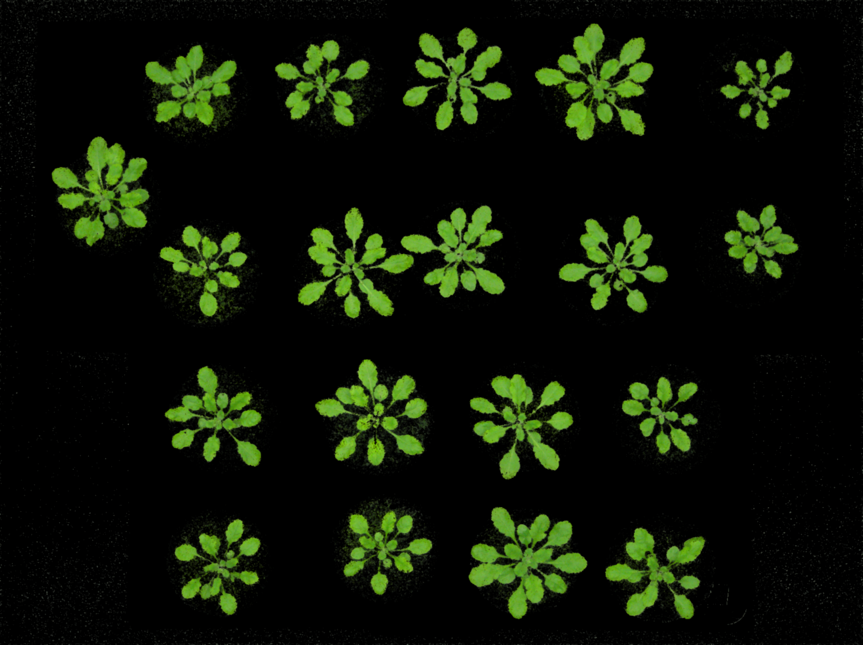
\includegraphics[scale=0.45]{T21.png}}
\caption{Sample pictures of intermediate process }
\label{fig1}
\end{figure}

\paragraph{}A new predicted bbox is obtained. AP is calculated by comparing the obtained bbox with the ground truth.

\subsection{Mask-RCNN}
There are three datasets, Ara2012, Ara2013-Canon, and Tobacco. The dataset was split 60\% to the training dataset, 20\% to the validation dataset, and 20\% to the test dataset. Also, all the test datasets will be involved in a new dataset namely: Dataset All, which is used to test the generalization ability. Experiments had been conducted on Google Colab. Used python packages are: opencv, skimage, tensorflow, keras and numpy. For Mask-RCNN, ResNet101 backbone with a feature pyramid network has been used. The dataset was split 60\% to the training dataset, 20\% to the validation dataset, and 20\% to the test dataset. This pre-trained model is trained by thousands of real plants images and synthetic plans images[6]

As well as the model was fine-tuned by training dataset and validation dataset, with training the network for 5 epoch with a random image. In order to train the model. we change the parameter. The batch size is four. The learning rate of the stochastic gradient descent optimizer is 0.001. The momentum is 0.9 and weight decay is 0.001. the batch size is four. 

The strengthen method was used. For all images, horizontally flip 50\% and vertically flip 50\%. Then, randomly cropping image by -25\% to 25\% of the height/ weight, then, scaling image to 80\% to 120\% of the size, rotating by 45 degrees, shearing 16 degrees. Then, using Gaussian blurring for all images, for which the kernel is 5. changing the brightness of per channel image and change hue and saturation from -20 to 20. there is a 50\% chance of each input image will be applied by each augmentation.



\section{Results}
\subsection{Plant Detection}

Input data: Ara2012:Tray/Ara2012/*\_rgb.png(16files),    \\ Tray/Ara2012/*\_bbox.csv (16 files)

The two methods of target detection for 16 images in the Ara2012 file yielded the AP results shown in the table I,
As well as the performance of two methods shown in Figure 2, which also has been proved in Figure 3.

\begin{figure*}[htbp]
\centerline{\includegraphics[scale=0.4]{T11.png}}
\caption{Example Results of Task1.}
\label{fig2}
\end{figure*}

\begin{table}[htbp]
\caption{ the AP results of 16 images in the Ara2012 file yielded}
\begin{center}
\begin{tabular}{|c|c|c|}

\hline
Image &HOG+SVM&Color Threshold \\
\hline
1&0.2545 &1.0 \\
\hline
2&0.4545 &1.0 \\
\hline
3&0.3409 &1.0 \\
\hline
4&0.6294 &1.0 \\
\hline
5&0.5289 &1.0 \\
\hline
6&0.6234 &1.0 \\
\hline
7&0.2545 &1.0 \\
\hline
8&0.8182 &1.0 \\
\hline
9&0.8182 &1.0 \\	
\hline
10&0.8182 &1.0 \\	
\hline
11&1.0000 &1.0 \\
\hline	
12&0.9091 &1.0 \\
\hline
13&0.9091 &1.0 \\	
\hline
14&0.8182 &1.0 \\	
\hline
15&1.0000 &1.0 \\	
\hline
16&0.9091 &1.0 \\
\hline
17&0.9091 &1.0 \\
\hline
\hline

\end{tabular}
\label{tab1}
\end{center}
\end{table}



\begin{table}[htbp]
\caption{Time Consuming of Different Methods}
\begin{center}
\begin{tabular}{|c|c|}

\hline
Methods &Time Consuming \\
\hline
HOG+SVM&19.797090  \\
\hline
Color Threshold&410.927392  \\
\hline

\end{tabular}
\label{tab2}
\end{center}
\end{table}


\begin{figure}[htbp]
\centerline{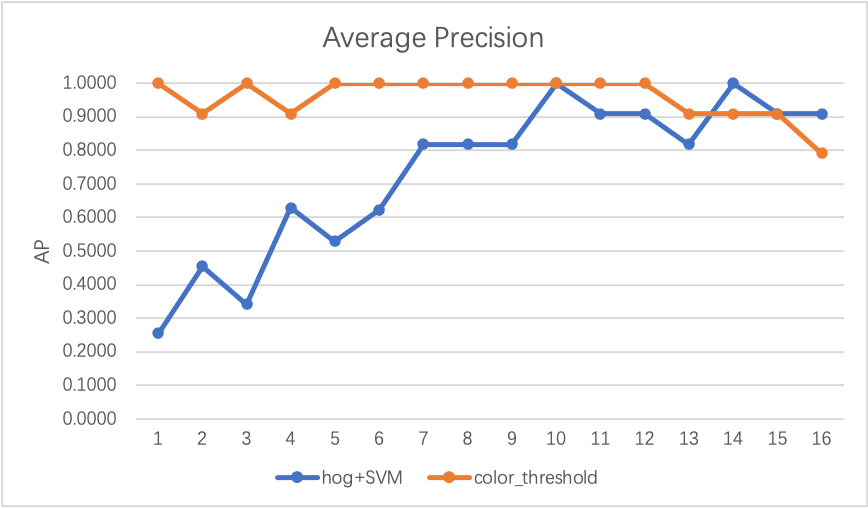
\includegraphics[scale=0.59]{P1.png}}
\caption{AP results of 16 images in the Ara2012 file yielded.}
\label{fig1}
\end{figure}






\begin{itemize}
\item When using non-maximum suppression, it is necessary to select a better threshold. Here, the threshold=0.06 was chosen.
\item The sample size and the selection of negative samples are important. The sample selection should be appropriate to the actual project environment to obtain the sample set. The initial attempt was to take a random screenshot of the image with the same number of negative and positive samples after reading the image data. The problem was that the sample selection was not comprehensive enough and still resulted in inaccurate testing. So the experiment is taking random samples and saving them, and then selecting them manually.
\item Different images end up with different results.  Especially when the plants are small, the detection does not work well. Consider whether to include more pictures of different smaller plants in the data of the positive sample.
\item Shorter running times. Faster results.
\end{itemize}

\subsection{Plant Segmentation}

\subsubsection{Color Space Formats}
Table III shows the comparison of Normalized RGB and HSV applied in image segmentation.
As it was shown, HSV format performs much better than RGB format,
which could also be proved by Figure 4,5.
\begin{table}[htbp]
\caption{Comparison of Normalized RGB and HSV}
\begin{center}
\begin{tabular}{|c|c|c|}

\hline
Methods&Normalized RGB &HSV \\
\hline
median DSC  &0.927510 &0.950156\\
\hline
median IOU &0.864818 &0.905046\\
\hline
average DSC  &0.904955 &0.948072\\
\hline
average IOU &0.830483 &0.901851\\
\hline
Time &135 &128\\
\hline

\end{tabular}
\label{tab3}
\end{center}
\end{table}



\begin{figure}[htbp]
\centerline{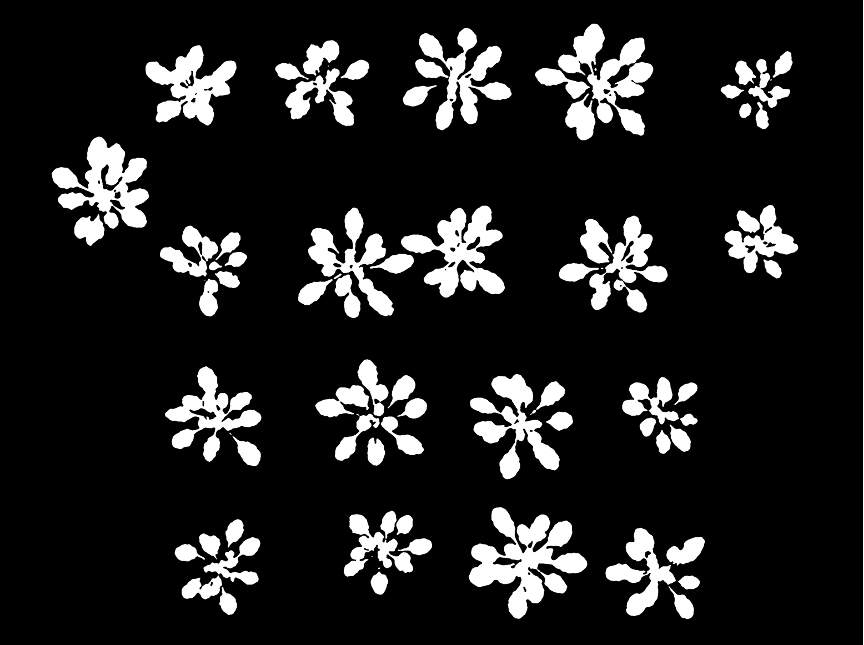
\includegraphics[scale=0.37]{T22.png}}
\caption{An example of the segmentation result applied HSV}
\label{fig3}
\end{figure}
\begin{figure}[htbp]
\centerline{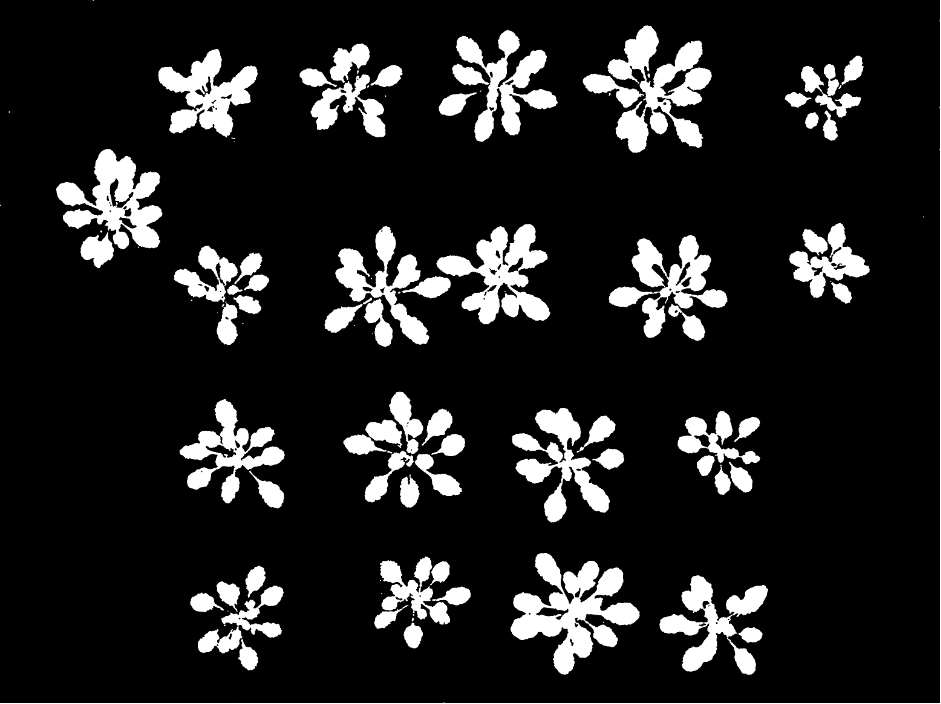
\includegraphics[scale=0.35]{T23.png}}
\caption{An example of the segmentation result applied RGB.}
\label{fig4}
\end{figure}



\subsubsection{ Segmentation Methods}
Table IV shows the comparison between image segmentation using kmeans method and pure threshold operation.
\begin{table}[htbp]
\caption{Comparison of three methods }
\begin{center}
\begin{tabular}{|c|c|c|c|}

\hline
Methods&Kmeans &Threshold& Watershed \\
\hline
median DSC  &0.9567&0.9325 & 0.9519\\
\hline
median IOU &0.9436 &0.8956   & 0.9050\\
\hline
average DSC  &0.9170 &0.8918 & 0.9492\\
\hline
average IOU &0.8947 &0.901851    & 0.9041\\
\hline
Time(s) &7468.3 &30.92&39.34\\
\hline

\end{tabular}
\label{tab4}
\end{center}
\end{table}

As shown in Table IV, the median DSC applied Kmeans is 0.951871,
and metric without Kmeans is 0.950156, as well as all other metrics of Kmeans 
are slightly greater than the traditional approaches, which should be considered with the time consuming,
Kmeans-clustering takes a horrible running time.

\begin{figure*}[htbp]
\centerline{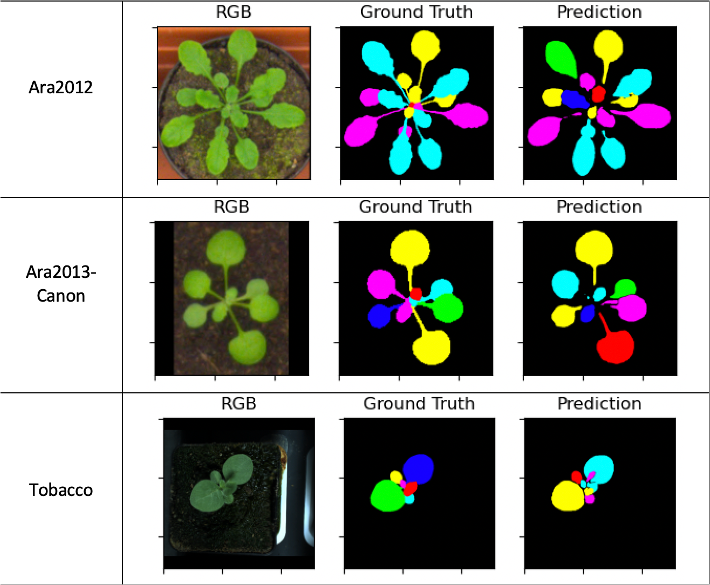
\includegraphics[scale=1.1]{T3.png}}
\caption{Example Results of Task3.}
\label{fig4}
\end{figure*}

\subsection{Individual Leaf Segmentation}
For qualitative evaluation, the leaf segmentation of each dataset are shown in Table V : 

In Figure 6, the leaf segments to different colors, each color present one leaf.

For quantitative evaluation, the performance evaluation table is shown below: 
The SBD is using in the experimental setup part.

\begin{table}[htbp]
\caption{Time Consuming of Different Methods}
\begin{center}
\begin{tabular}{|c|c|c|c|c|}

\hline
Methods&Ara2012 &Ara2013-Canon&Tobacco&ALL \\
\hline
Mask-R-CNN &&&&\\
+ResNet50&74.4157 &77.3661&42.2667&74.1102  \\
+FPN+SVM &&&&\\
\hline
Mask-R-CNN&&&&\\
+ResNet101&77.5184&79.7582&61.5986&79.9511 \\
+FPN&&&&\\
\hline

\end{tabular}
\label{tab5}
\end{center}
\end{table}

The performance in Dataset Ara2012 is the best. The SBD of Dataset Ara2013-Canon is lower than Dataset ara2012 because the moss on the ground may affect the result. 
The SBD of tobacco is the lowest. There are three reasons:
The first one is the dataset of tobacco is the smallest. 
The second one is some of the tobacco images is too small, which the SBD score is 0 because the leaf area is too small to find.
The third one may because the pixel value of tobacco images is much higher, the texture of leaves may deeper, leading to over-segmentation while training, which could be seen in Figure 7.




\begin{figure}[htbp]
\centerline{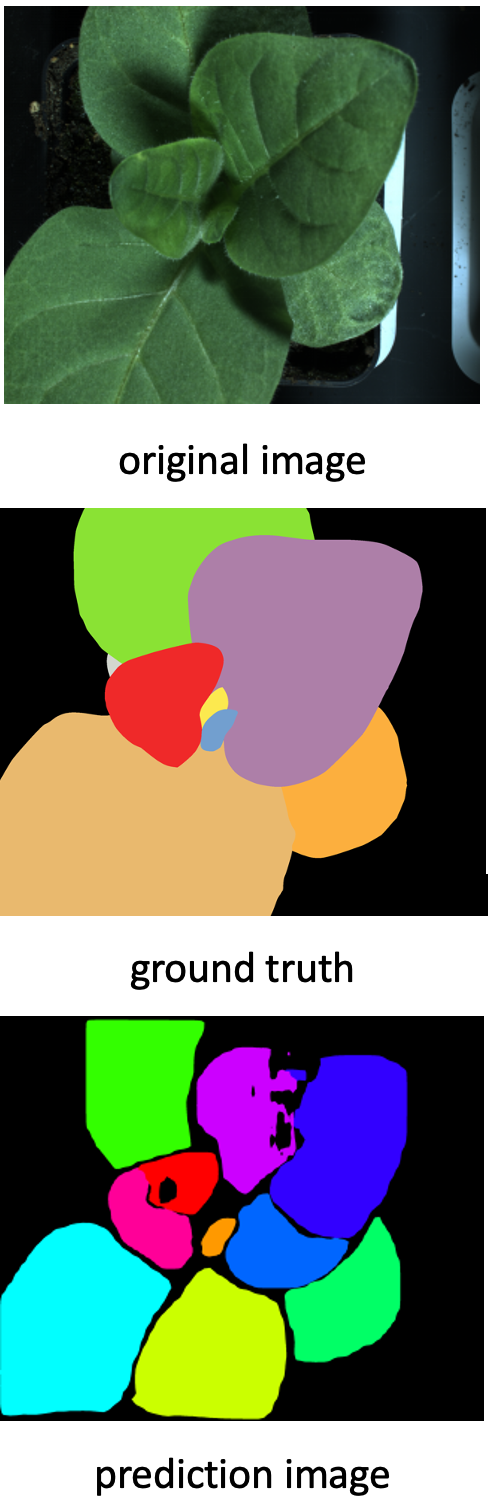
\includegraphics[scale=0.55]{T33.png}}
\caption{Sample pictures of intermediate process }
\label{fig7}
\end{figure}

The SBD of Mask-R-CNN with ResNet101 is higher than Mask-R-CNN with ResNet50, although the improvement is not obvious. The performance on tobacco image is much better while using Mask-R-CNN with ResNet101. The Mask-R-CNN with ResNet101 could be used to get a better result.

\section{Discussion and Conclusions}
\subsection{HOG+SVM}



\begin{itemize}
\item HOG+svm requires a large number of positive and negative samples, and the samples need to be selected as closely as possible to the actual project environment.
\item The two methods are fundamentally different. HOG+svm is machine learning, and color thresholds are the traditional method.
\item Hog+svm is used for the same type of object detection, such as pedestrian detection. Color thresholds are used for target detection and localization of monochromatic objects.
\item Hog+svm takes a short time, while the color threshold takes a long time. However, the performance of the former is very poor for detecting smaller plants and good for detecting larger plants. The color threshold method is less affected by the plant size.
\item Using Hog+svm for detection, the final resultant boxes are of fixed size scale and do not change with the size of the plant. Therefore, the predicted frames deviate more from the plant ground truth frames. The box drawn using the color threshold method will change with the shape of the plant.
\end{itemize}


\subsection{Preprocessing}
\begin{itemize}
\item In the pre-processing section, if much noise is removed, then the rhizomes of finer plants can be mistaken for noise and removed. A disconnection between leaves of the same plant.
\item When getting the first rough bbox prediction, some labels with a very small number of labels are removed. This can actually be seen as manual noise removal.
\item If two plants are too close together or if the leaves of two plants overlap, it is very easy to assume that they are the same plant. Although it is possible to locate the plant, it can affect the determination of the number of plants.
\item Uses traditional methods, so the pixels of the image are traversed multiple times during the run. The time complexity is high and the run time is long.
\end{itemize}

\begin{figure}[htbp]
\centerline{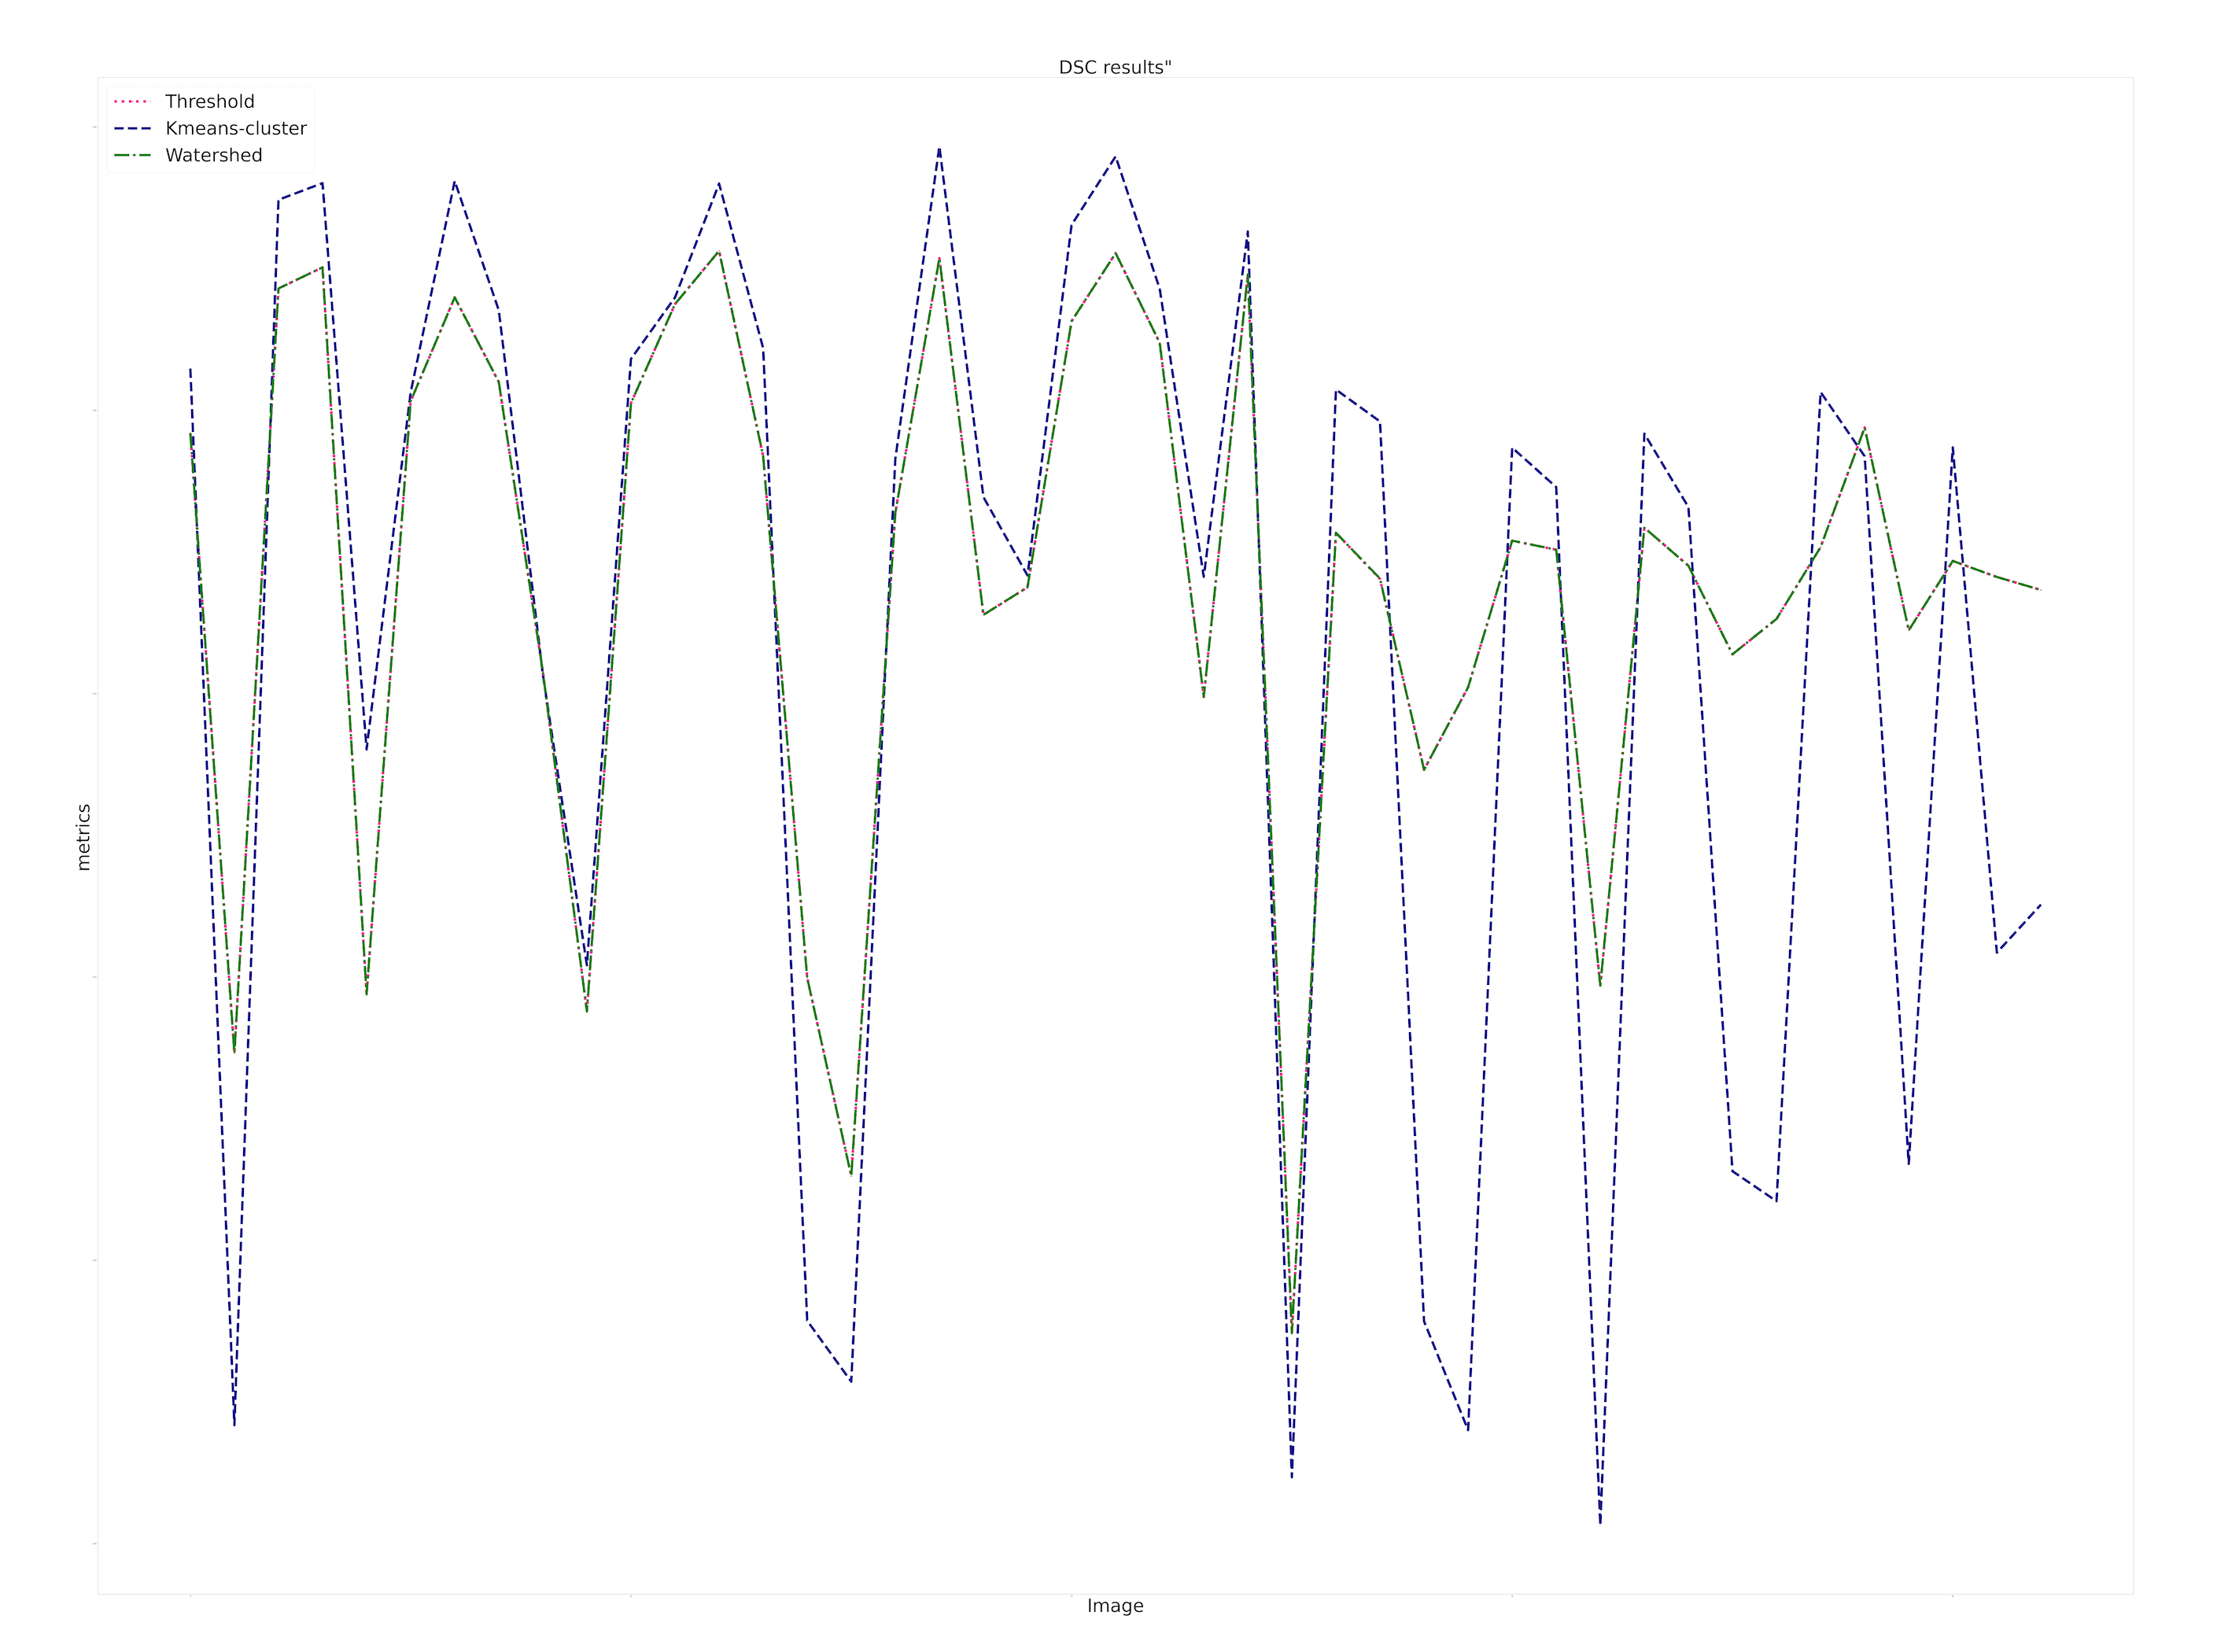
\includegraphics[scale=0.15]{DSC.png}}
\caption{Sample pictures of intermediate process }
\label{fig8}
\end{figure}

\begin{figure}[htbp]
\centerline{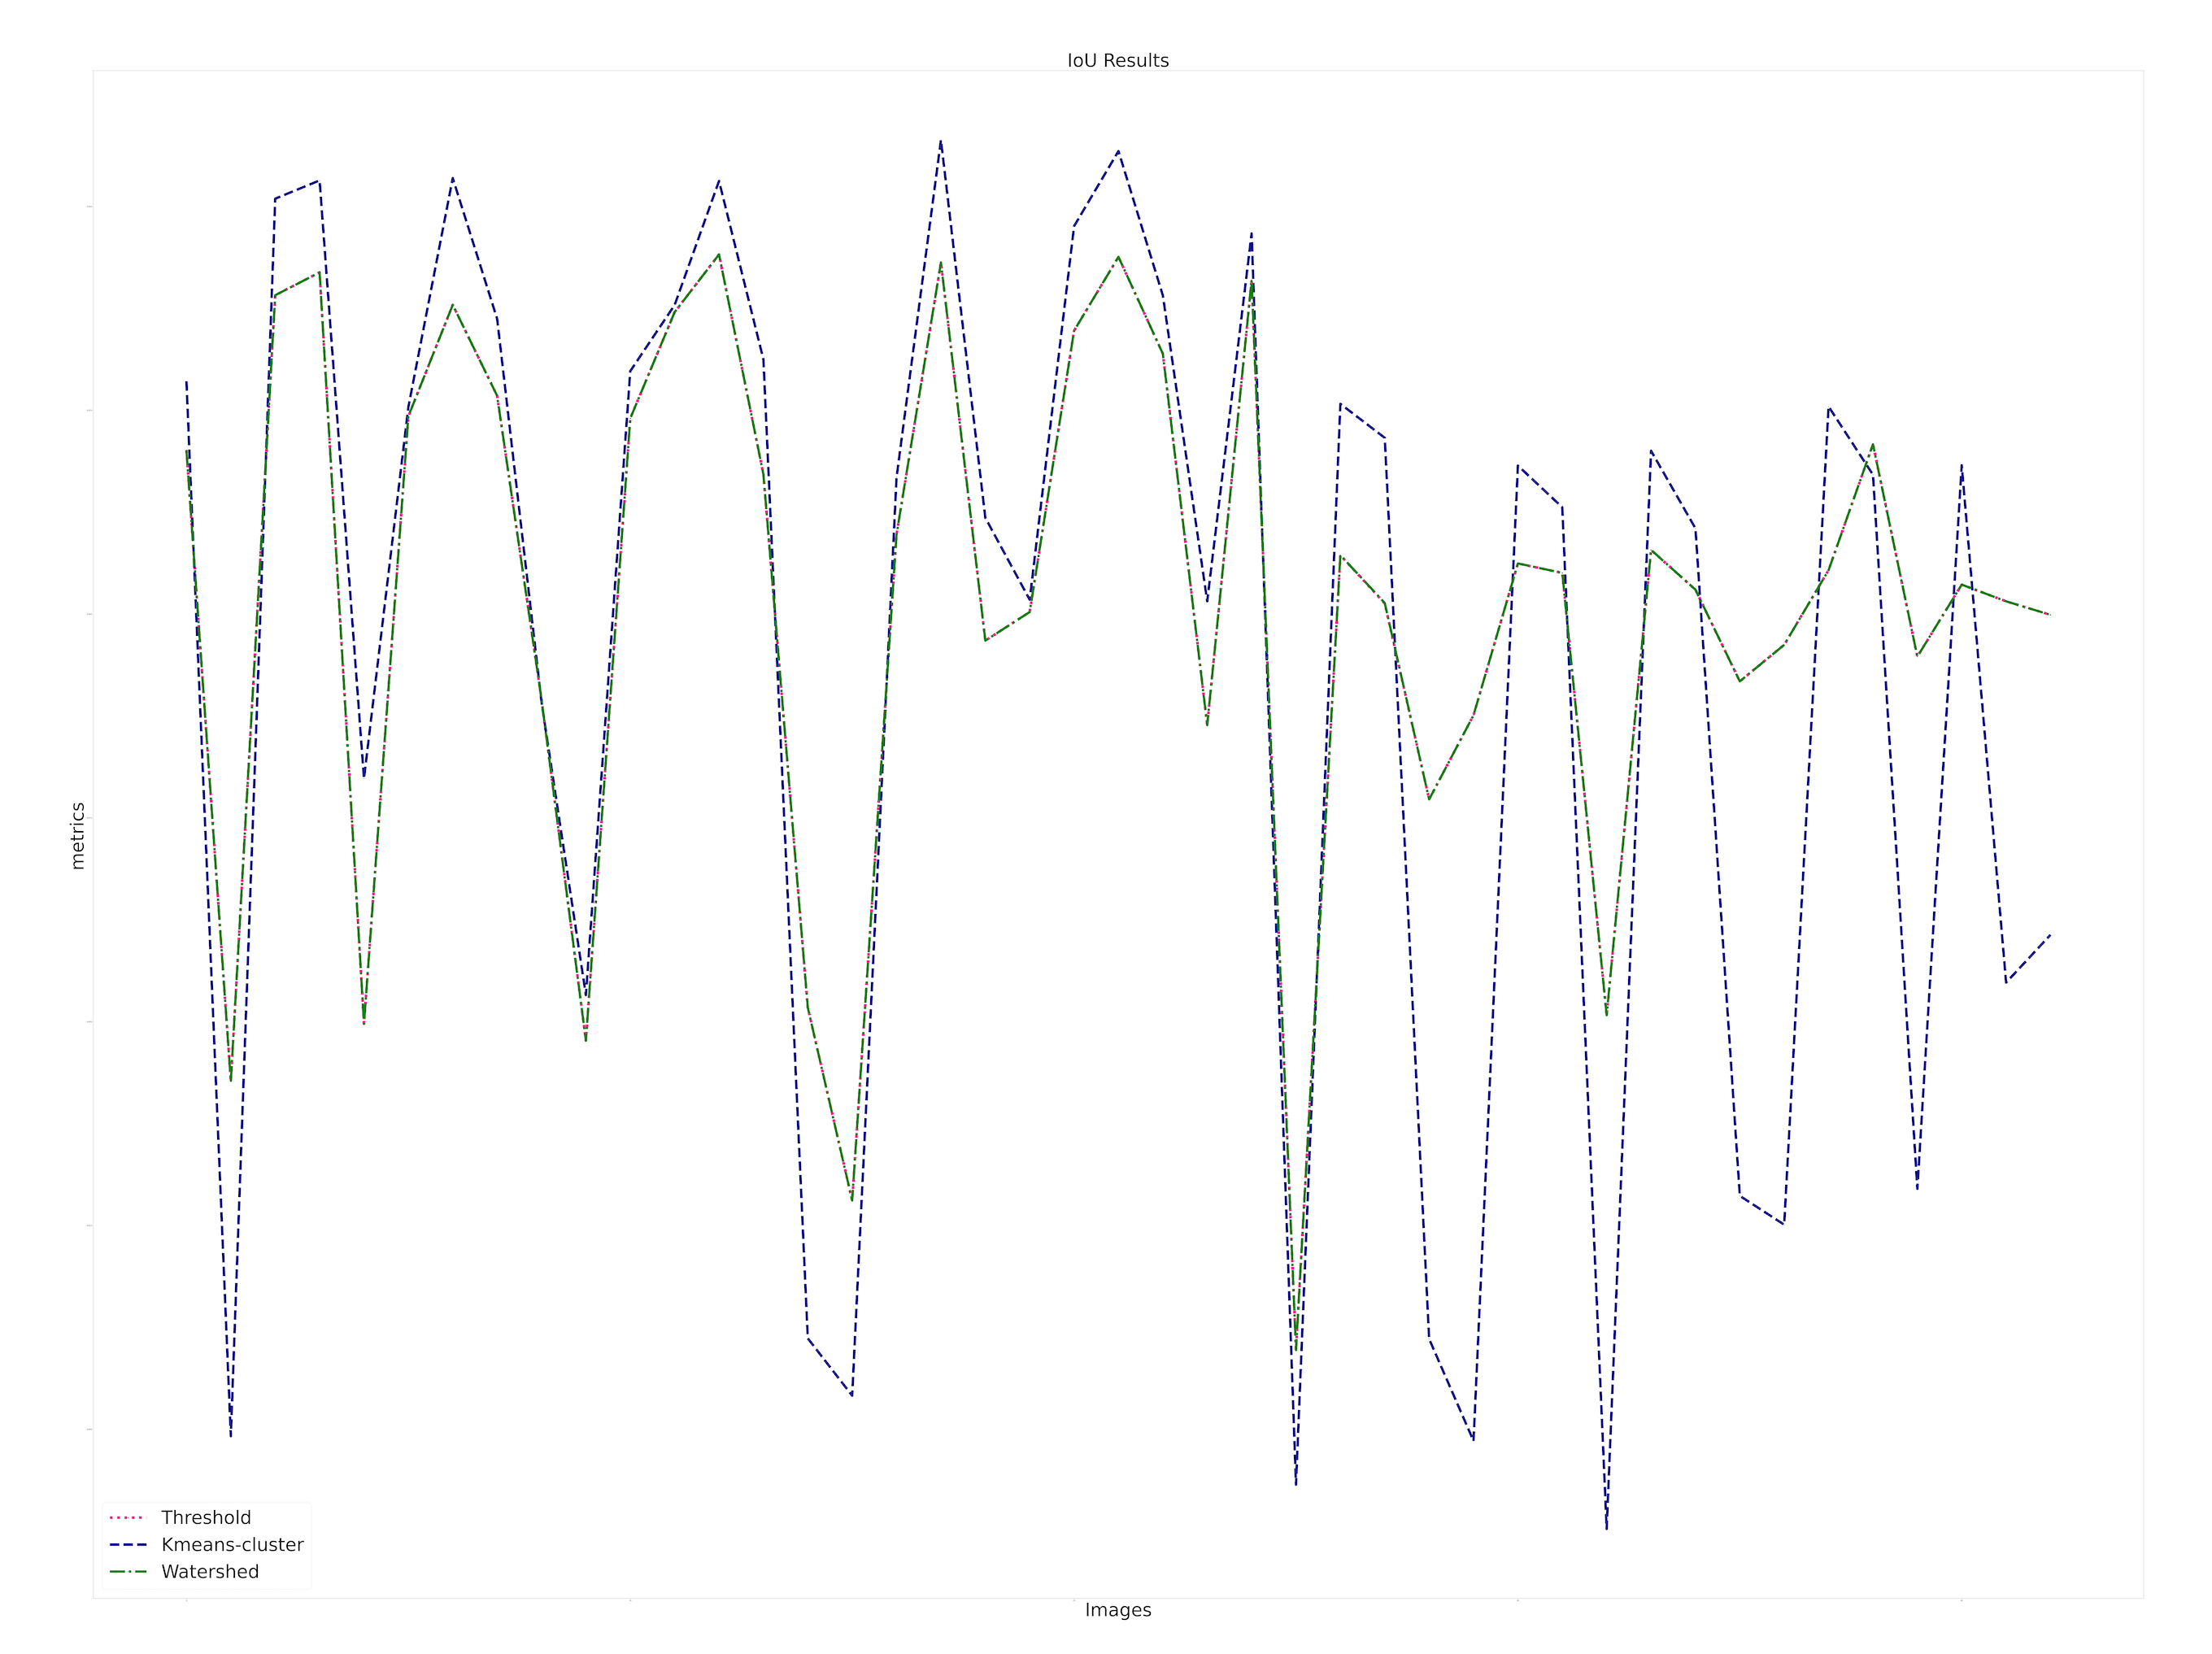
\includegraphics[scale=0.15]{IOU.png}}
\caption{Sample pictures of intermediate process }
\label{fig9}
\end{figure}

\subsection{Kmeans and Watershed}
As results of the comparison of three segmentation methods shown in Table IV, Figure 8, 9 are the metrics shown by plots.

As they show, the watershed and K-means performed better.
for the Dice Similarity Coefficient, K-means gets higher scores, and watershed gets higher in Intersection Over Union,
For the reasons
When we have an inspection on the best performance image and the worst,
it may be because the Dice Similarity Coefficient concentrate more on the True Positive part instead of Intersection Over Union
And K-means performs better on removing the noisy item,
which removed the edge of the tray but other methods could not make it.
In addition, iterations K-means iterations blurred edges of leaves.

In conclusion, when the target datasets are not too large, K-means performs better, otherwise, watershed segmentation should be considered.

\subsection{Mask-R-CNN}
The performance of the deep learning method is good, but there still have space to improve. Because of the time limit, the model just gets trained with three epochs. To increase the number of epoch to improve the model should be considered next. The model performance should be improved to detect small leaf. The model could use Mask-R-CNN with ResNet50 to reduce the time since the result is not obviously different between Mask-R-CNN+ResNet50 and Mask-R-CNN+ResNet101.
\section{Contribution of Group Members}
Below are the contribution of all group members, each member made equal contributions in the presentation and demonstration. 
\begin{itemize}

\item Tianyi Wu (z5263505):
Read the reference documents. 
Code for Task 1. 
Finished the methods, experimental setup, and results of task 1. \\

\item Siyu Gao (z5251491):
Read the reference documents. 
Code for preprocessing images. 
Finished Intro, literature review, all typesetting, and layout of the whole report.\\


\item Xiaole Du (z5192402):
Read the reference documentss. 
Finished the methods, experimental setup, results, and conclusion of task 3, \\


\item Gewei Cheng (z5243425):
Read the reference documents. 
Code for Task 3. Integration of all codes.
Finished the results part in task 3.\\


\item Lijun Zhong (z5243425):
Read the reference documents. 
Code for Task 2. 
Finished the methods, experimental setup, results, and conclusion of task 2.\\
\end{itemize}

\begin{thebibliography}{00}

\bibitem{b1} N. Dalal and B. Triggs, “Histograms of oriented gradients for human detection,” in Computer Vision and Pattern Recognition, 2005. CVPR 2005. IEEE Computer Society Conference on, vol. 1, June 2005, pp. 886 –893 vol. 1.
\bibitem{b2} D. Ward, P. Moghadam, and N. Hudson, “Deep Leaf Segmentation Using
Synthetic Data,” ArXiv180710931 Cs, Jul. 2018.
\bibitem{b3} Massimo Minervini, Andreas Fischbach, Hanno Scharr, Sotirios A. Tsaftaris, Finelygrained annotated datasets for image-based plant phenotyping, Pattern Recognition Letters, Volume 81, 2016, Pages 80-89, ISSN 0167-8655
\bibitem{b4} Bert De Brabandere, Davy Neven, and Luc Van Gool. Semantic instance segmentation with a discriminative loss function. CoRR, abs/1708.02551, 2017.
\bibitem{b5} J.-M. Pape and C. Klukas. 3-D Histogram-Based Segmentation and Leaf Detection for Rosette Plants, pages 61–74. Springer International Publishing, Cham, 2015.
\bibitem{b6} He, K., Gkioxari, G., Dollar, P., Girshick, R., 2017. Mask R-CNN, in: 2017 ´IEEE International Conference on Computer Vision (ICCV), pp. 2980–2988.
\bibitem{b7} Ward, D., Moghadam, P. (2020). Scalable learning for bridging the species gap in image-based plant phenotyping. Computer Vision and Image Understanding, 103009.
\bibitem{b8} Wu, Q., Chen, Y., Meng, J.: Dcgan based data augmentation for tomato leaf disease identification. IEEE Access (2020)
\bibitem{b9} Tapas, A.: Transfer learning for image classification and plant phenotyping. International Journal of Advanced Research in Computer Engineering and Technology (IJARCET) 5(11), 26642669 (2016)
\bibitem{b10} M. Hiromoto and R. Miyamoto, “Hardware architecture for high-accuracy real-time pedestrian detection with CoHOG features,” in Computer Vision Workshops (ICCV Workshops), 2009 IEEE 12th International Conference on, 27 2009-Oct. 4 2009, pp. 894 –899.
\bibitem{b11} W. Zhang, G. Zelinsky, and D. Samaras, “Real-time accurate object detection using multiple resolutions,” in Proc. Int. Conf. Comput. Vision, 2007, pp. 1–8.
\bibitem{b12} De Vylder, J., Vandenbussche, F.J., Hu, Y., Philips, W., Van Der Straeten, D.: Rosette Tracker: an open source image analysis tool for automatic quantification of genotype effects. Plant Physiol. 60(3), 1149–1159 (2012)
\bibitem{b13} Hartmann, A., Czauderna, T., Hoffmann, R., Stein, N., Schreiber, F.: HTPheno: an image analysis pipeline for high-throughput plant phenotyping. BMC Bioinform. 12(1), 148 (2011)
\bibitem{b14}  Minervini, M., Abdelsamea, M.M., Tsaftaris, S.A.: Image-based plant phenotyping with incremental learning and active contours. Ecol. Inform. 23, 35–48 (2014). (Special Issue on Multimedia in Ecology and Environment)
\bibitem{b15} Vincent, L., Soille, P.: Watersheds in digital spaces: an efficient algorithm based on immersion simulations. IEEE Trans. Pattern Anal. Mach. Intell. 13(6), 583–598 (1991)
\bibitem{b16} Wan-Ting Lin, Chuen-Horng Lin, Tsung-Ho Wu, and YungKuan Chan, Image Segmentation Using the K-means Algorithm for Texture Features, World Academy of Science, Engineering and Technology, 65, 2010. 
\bibitem{b17} Jarosław Gocławski, An Automatic Segmentation Method for Scanned Images of Wheat root Systems with Dark Discolourations, Int. J. Appl. Math. Comput. Sci., Vol. 19, No. 4, pp.679–689, 2009. 
\bibitem{b18} Nor Ashidi Mat Isa, " Automated Edge Detection Technique for Pap Smear Images Using Moving K-Means Clustering and Modified Seed Based Region Growing Algorithm", International Journal of The Computer, the Internet and Management Vol. 13.No.3 ,pp 45-59, 2005. 
\bibitem{b19} Rafael C.Gonzalez, Richard E.Woods, Steven L.Eddins, “Digital Image Processing”, Pearson Education, 2nd Edition. 

\end{thebibliography}



\end{document}
